\documentclass[11pt]{article}
\usepackage[T1]{fontenc}
\usepackage[utf8]{inputenc}
\usepackage{lmodern,microtype,amsmath,amssymb,amsthm,mathtools,mathrsfs}
\usepackage[margin=30mm]{geometry}
\usepackage{booktabs,enumitem,tikz,xcolor,xurl}
\usetikzlibrary{arrows.meta,positioning,calc}
\usepackage[unicode,colorlinks=true,linkcolor=blue!45!black,urlcolor=blue!55!black,citecolor=green!35!black]{hyperref}
\setlength{\emergencystretch}{2em}
\numberwithin{equation}{section}
\newtheorem{theorem}{Theorem}[section]
\newtheorem{proposition}[theorem]{Proposition}
\newtheorem{lemma}[theorem]{Lemma}
\newtheorem{corollary}[theorem]{Corollary}
\theoremstyle{definition}\newtheorem{definition}[theorem]{Definition}
\theoremstyle{remark}\newtheorem{remark}[theorem]{Remark}
\newcommand{\ii}{\mathrm i}\newcommand{\dd}{\mathrm d}
\newcommand{\CC}{\mathbb C}\newcommand{\RR}{\mathbb R}\newcommand{\ZZ}{\mathbb Z}
\newcommand{\cH}{\mathcal H}\newcommand{\Bhat}{\widehat B}
\newcommand{\Turn}{\mathsf T}\newcommand{\Cheb}{\mathsf C}
\newcommand{\Tr}{\operatorname{Tr}}\newcommand{\arccot}{\operatorname{arccot}}
\newcommand{\eps}{\varepsilon}
\title{Newton coefficients and positive sources for Conway tangles}
\author{}\date{}
\begin{document}\maketitle
\begin{abstract}
At a principal root of unity, the two-strand Casimir has repeated
spectral roots. We construct a Newton basis in its full polynomial
algebra and prove exact formulas for multiplication, the physical
quarter-turn, closure and colored crossing circles. The formulas retain
the derivative data at repeated roots. The complete-circle coefficients
are positive, and multiplication has an explicit positive integer
support. For a specified class of finite Conway compositions, we prove
that the logarithmic growth of the complete auxiliary-color source is
the maximum of a strictly concave action on a primitive lattice
polytope. The maximum lies in its strict interior at both level
parities. An exact recursion for the output derivative places every
stationary leaf parameter in a fixed interval above one quarter.
These results provide finite and variational inputs for estimates of
signed fillings; the positive auxiliary source is the object whose
limit is proved here.
\end{abstract}

\section{Introduction}
A tangle calculation changes character when two spectral roots
coincide. Polynomial values alone no longer determine the operator:
a derivative can multiply a nonzero nilpotent matrix. This paper uses
one polynomial algebra throughout the tangle calculation, keeping both
values and first derivatives. Its basis is chosen so that a physical
quarter-turn reverses the basis index. Multiplication then has positive
coefficients with a simple support, and cylindrical closure pairs
complementary indices.

The exact identities are useful beyond their individual formulas.
They turn a recursively composed tangle into a finite sum over integer
indices, with no intermediate division by a vanishing spectral
factor. For the complete color on every auxiliary circle, each
nonzero summand is positive. We identify its exponential rate and prove
that the maximizing state stays away from every boundary not forced
by closure. The proof includes the integer rounding needed to pass
through every sufficiently large level, rather than only levels in a
chosen congruence class.

The two principal conclusions are the exact basis calculus in
Proposition~\ref{prop:newton-turn} and Theorem~\ref{thm:positive-product},
and the positive-source theorem in Proposition~\ref{prop:strict-maximum}
and Corollary~\ref{cor:complete-limit}. Lemma~\ref{lem:port-bounds}
adds a quantitative interval for the stationary leaf coordinates.
The construction and all its leaves are fixed before the level grows.
A complete source still has to be compared with the signed contributions
and with the entire filling sum before it gives a volume theorem.

Kashaev's crossing-matrix definition supplies the knot-theoretic
background \cite{Kashaev1995}. The exact enhanced normalization used
here is the one compared with that definition in \cite[Theorem~10.1]{Finite}.
The present paper proves the additional Newton and turn formulas used
for composition. Rational-tangle conventions are discussed in
\cite{KauffmanLambropoulou}; our endpoint order is fixed below.
The variational argument uses the elementary tetrahedron-volume
concavity appearing in the Casson--Rivin approach, for which
\cite{FuterGueritaud} provides an exposition. Here the positive source,
its polytope and its boundary argument are established directly;
construction of a complete hyperbolic metric is a separate problem.

\section{The diagrams and the positive source}\label{nt:diagrams}
A two-string tangle consists of two arcs in a ball with four prescribed
boundary points. Additional closed curves are allowed and will include
the auxiliary crossing circles. Label the exposed endpoints in their
cyclic order by
\[
0=\text{bottom left},\quad1=\text{bottom right},\quad
2=\text{top right},\quad3=\text{top left}.
\]
For a vertical stack $FG$, place $F$ below $G$ and join $F_2$ to $G_1$
and $F_3$ to $G_0$. The exposed tuple is $(F_0,F_1,G_2,G_3)$.
A clockwise quarter-turn carries the entire tangle with its box; the
new tuple is $(F_1,F_2,F_3,F_0)$ in terms of the old labels.
Cylindrical closure $C(FG)$ joins the remaining bottom and top endpoints
on each side, without additional crossings. These connections are shown
in Figure~\ref{nt:operations}.

\begin{figure}[ht]
\centering% Ordered boundary connections; boxes suppress their interior tangles.
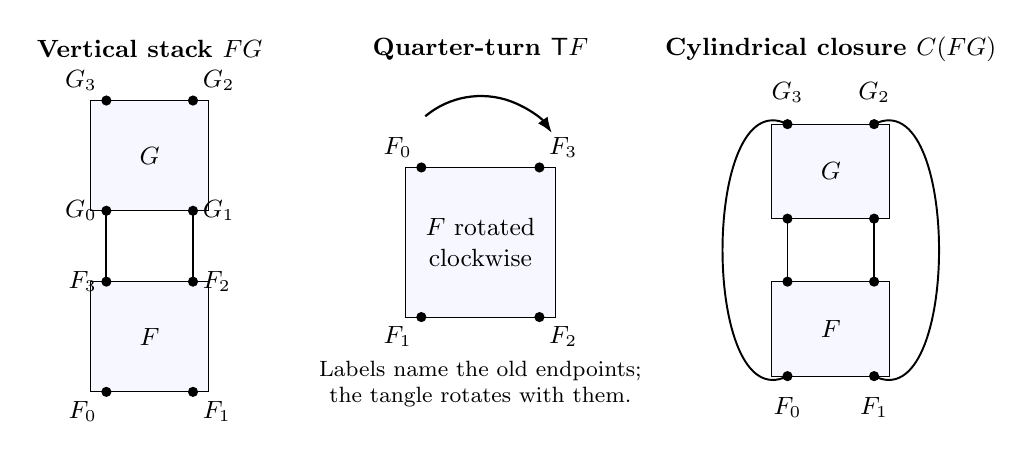
\begin{tikzpicture}[x=1cm,y=1cm, every node/.style={font=\small},
 tangent/.style={line width=.7pt}, terminal/.style={circle,fill=black,inner sep=1.3pt}]
% Left: stacking.
\begin{scope}[shift={(0,0)}]
 \node[font=\small\bfseries] at (1.2,4.8) {Vertical stack $FG$};
 \draw[fill=blue!3] (.45,.45) rectangle (1.95,1.85);
 \draw[fill=blue!3] (.45,2.75) rectangle (1.95,4.15);
 \node at (1.2,1.15) {$F$}; \node at (1.2,3.45) {$G$};
 \foreach \x in {.65,1.75} {
  \draw[tangent] (\x,1.85)--(\x,2.75);
  \foreach \y in {.45,1.85,2.75,4.15} \node[terminal] at (\x,\y) {};
 }
 \node[below left] at (.65,.45) {$F_0$};\node[below right] at (1.75,.45) {$F_1$};
 \node[left] at (.65,1.85) {$F_3$};\node[right] at (1.75,1.85) {$F_2$};
 \node[left] at (.65,2.75) {$G_0$};\node[right] at (1.75,2.75) {$G_1$};
 \node[above left] at (.65,4.15) {$G_3$};\node[above right] at (1.75,4.15) {$G_2$};
\end{scope}
% Middle: a genuine clockwise turn, showing old labels in new positions.
\begin{scope}[shift={(4.25,0)}]
 \node[font=\small\bfseries] at (1.15,4.8) {Quarter-turn $\mathsf T F$};
 \draw[fill=blue!3] (.2,1.4) rectangle (2.1,3.3);
 \node[align=center] at (1.15,2.35) {$F$ rotated\\clockwise};
 \foreach \p in {(.4,1.4),(1.9,1.4),(1.9,3.3),(.4,3.3)} \node[terminal] at \p {};
 \node[below left] at (.4,1.4) {$F_1$};\node[below right] at (1.9,1.4) {$F_2$};
 \node[above right] at (1.9,3.3) {$F_3$};\node[above left] at (.4,3.3) {$F_0$};
 \draw[-{Latex[length=2mm]},thick] (.45,3.95) arc[start angle=130,end angle=35,radius=1.1];
 \node[align=center,font=\footnotesize] at (1.15,.55) {Labels name the old endpoints;\\the tangle rotates with them.};
\end{scope}
% Right: closure arcs are actual identity connections outside both boxes.
\begin{scope}[shift={(8.65,0)}]
 \node[font=\small\bfseries] at (1.2,4.8) {Cylindrical closure $C(FG)$};
 \draw[fill=blue!3] (.45,.65) rectangle (1.95,1.85);
 \draw[fill=blue!3] (.45,2.65) rectangle (1.95,3.85);
 \node at (1.2,1.25) {$F$};\node at (1.2,3.25) {$G$};
 \foreach \x in {.65,1.75} {
  \draw[tangent] (\x,1.85)--(\x,2.65);
  \foreach \y in {.65,1.85,2.65,3.85} \node[terminal] at (\x,\y) {};
 }
 \draw[tangent] (.65,.65)..controls(-.45,.1)and(-.45,4.4)..(.65,3.85);
 \draw[tangent] (1.75,.65)..controls(2.85,.1)and(2.85,4.4)..(1.75,3.85);
 \node[below] at (.65,.5) {$F_0$};\node[below] at (1.75,.5) {$F_1$};
 \node[above] at (.65,4.0) {$G_3$};\node[above] at (1.75,4.0) {$G_2$};
\end{scope}
\end{tikzpicture}

\caption{Stacking, clockwise rotation and cylindrical closure. Each box
contains its entire tangle. The outside arcs specify the actual
connections used in the evaluation.}\label{nt:operations}
\end{figure}

Let $L_j$ be an auxiliary circle carrying the $j$-dimensional
highest-weight representation and surrounding two main strands of
complete color $N$. Its disk fixes the ordering and framing. Set
$h_j=\Turn L_j$. When discussing the construction, $h$ denotes one
such turned circle; in the positive source it is evaluated as $h_N$.
Every written occurrence is a distinct auxiliary circle.

\begin{definition}[Completed expressions]\label{def:grammar}
Start with the stack $hh$. One may turn a constructed box, stack two
constructed boxes, or attach a single elementary piece on either side.
Equivalently,
\[
 E::=hh\mid\Turn(E)\mid E_1E_2\mid hE\mid Eh.
\]
A closed expression is $C(FG)$ with both $F$ and $G$ completed.
The word ``completed'' specifies this rule; it has no metric meaning.
\end{definition}

The positive complete source $Z_{F,G,N}$ is the cylindrical evaluation
of this fixed expression when every elementary piece is $h_N$, with
no retained half twists. Section~\ref{nt:algebra} defines that scalar
as $\phi(FG)$ in the physical pair algebra. Thus it is an explicit
finite tangle evaluation before any auxiliary filling. There is no
assumption here that its closed main strands form a knot. If the source
is later used in a knot application, its endpoint pairing and filling
conventions must be checked in that application.

For example, $C((hh)(hh))$ has four leaves, and
$C((h\Turn(hh))(hh))$ has five. The rule allows both branching and
nesting. Its requirement on the two closing children is used in the
proof of Lemma~\ref{lem:port-bounds}; a single bare closing leaf is
outside the theorem.

\section{The physical pair algebra}\label{nt:algebra}
Fix $N\ge2$, and set
\begin{equation}\label{eq:root-notation}
 d=N-1,\qquad q=e^{\pi\ii/N},\qquad Q=q^2,\qquad
 x=q^d,\qquad \kappa=q^{d^2/2},\qquad \rho=q-q^{-1}.
\end{equation}
There is no restriction to prime or odd $N$. The main strands carry the $N$-dimensional vector space $V_N$; this is what ``complete color'' means at this stage. The operators $H,K,E,F$ encode its quantum-group action. They are concrete matrices, which we specify so that the crossing convention can be checked. One convenient choice of basis is $v_0,\ldots,v_d$ and
\[
 H v_j=(d-2j)v_j,\quad K=q^H,\quad
 E v_j=[j]_q^2v_{j-1},\quad Fv_j=v_{j+1},
 \qquad [j]_q=\frac{q^j-q^{-j}}{q-q^{-1}}.
\]
Missing endpoint vectors are zero. For $k\ge0$, the quantum factorial is
$[k]_q!=\prod_{r=1}^k[r]_q$, with $[0]_q!=1$.
The finite universal crossing, including its Cartan factor, is
\begin{equation}\label{eq:universal-crossing}
 \mathscr R=q^{H\otimes H/2}
 \sum_{k=0}^{d}\frac{q^{k(k-1)/2}\rho^k}{[k]_q!}
 E^k\otimes F^k.
\end{equation}
Every denominator is nonzero. The physical braided crossing is obtained with the fixed exchange and transpose convention; the inverse is the actual matrix inverse. The framing and enhancement are part of the definition, not an unspecified factor appended to an asymptotic formula.

For calculations in the polynomial algebra it is useful to change basis on this same space. We call the new coordinates balanced; they do not define a different invariant. In this basis the operators are
\begin{equation}\label{eq:balanced-module}
 \mathcal E|a\rangle=(Q^{-a}-1)|a-1\rangle,\quad
 \mathcal F|a\rangle=(1-Q^{a+1})|a+1\rangle,\quad
 K|a\rangle=xQ^{-a}|a\rangle.
\end{equation}
The ordinary cup and cap, and the one marked cap, have entries
\begin{equation}\label{eq:cups}
 p_{ab}=Nx^{-b}\delta_{a+b,d},\qquad
 \ell_{ab}=\frac{x^a}{N}\delta_{a+b,d},\qquad
 m_{ab}=\frac{x^b}{N^2}.
\end{equation}
The cup creates two endpoints and the cap joins them. Their two snake identities say that a bend followed by the opposite bend evaluates to a straight strand. The different marked cap implements the reduced invariant and satisfies $mp=1$. The diagonal operator $g=K^{1-N}=(-1)^dK$ is the \emph{pivot}, the correction inserted when an ordinary strand is closed by a trace. For a two-strand operator $A$ commuting with the pair quantum-group action, the original cylindrical evaluation is
\begin{equation}\label{eq:phi-physical}
 \phi(A)=\frac1N\Tr_{V_N\otimes V_N}\bigl[(I\otimes g)A\bigr].
\end{equation}
The factor $1/N$ in this expression is the single cut average. It is not repeated at the auxiliary circles.


In the ordinary highest-weight basis above, put
$p_a=\prod_{j=1}^a(1-Q^j)$. The balanced basis is
$|a\rangle=\rho^a p_a^{-1}v_a$, with
$\mathcal E=\rho E$ and $\mathcal F=\rho F$.
All $p_a$ with $a<N$ are nonzero. This gives an explicit diagonal
change of basis on the same representation. Its factors cancel on
contracted wires. The invariant normalization and crossing comparison
are those of \cite[Theorem~10.1]{Finite}; no asymptotic bound on this
change of basis is used.

\subsection{The full pair algebra}

An operator on two strands must commute with the joint action of the quantum-group generators if it is to represent one of our invariant tangle boxes. The formulas below specify that joint action. The subsequent lemma identifies all such commuting operators; this is the meaning of the term \emph{commutant}.
The balanced pair generators and Casimir are
\begin{equation}\label{eq:pair-casimir}
 \mathcal E_{12}=\mathcal E_1K_2+\mathcal E_2,\quad
 \mathcal F_{12}=\mathcal F_1+K_1^{-1}\mathcal F_2,\quad
 K_{12}=K_1K_2,\quad
 \Omega=\mathcal F_{12}\mathcal E_{12}+qK_{12}+q^{-1}K_{12}^{-1}.
\end{equation}
Let $\Cheb_n(z)=2T_n(z/2)$, where $T_n$ is the usual Chebyshev polynomial. Thus $\Cheb_0=2$, $\Cheb_1=z$ and $\Cheb_{n+1}=z\Cheb_n-\Cheb_{n-1}$. Define
\begin{equation}\label{eq:hermite-algebra}
 P_N(z)=\Cheb_N(z)+2=\prod_{j=0}^{d}(z-c_j),\qquad
 c_j=q^{2j+1}+q^{-2j-1},\qquad
 \cH_N=\CC[z]/(P_N).
\end{equation}
The list of roots includes multiplicity. Since $c_{d-j}=c_j$, all distinct roots are double except the simple root $-2$ at odd $N$.

\begin{lemma}[Full commutant]\label{lem:commutant}
The endomorphisms of $V_N\otimes V_N$ commuting with the three pair generators are exactly $\CC[\Omega]\simeq\cH_N$.
\end{lemma}
\begin{proof}
Let $W_T$ be the span of $|a,T-a\rangle$. The $K_{12}$ eigenvalue one occurs only on $W_d$. The matrices $\mathcal E_{12}:W_{T+1}\to W_T$ for $T<d$, and $\mathcal F_{12}:W_T\to W_{T+1}$ for $T\ge d$, have triangular maximal minors with nonzero diagonals. Consequently the entire pair is generated from $W_d$ by these raising and lowering operators.

On $W_d$, the Casimir is a symmetric tridiagonal matrix with adjacent entries $-(1-Q^{a+1})^2\ne0$. Its first basis vector is cyclic: the $k$th power has last possible coordinate $k$, with coefficient equal to the nonzero product of the first $k$ adjacent entries. An operator commuting with this block is therefore a unique polynomial of degree below $N$ in that block. Subtracting the same polynomial in $\Omega$ from a pair intertwiner gives zero on $W_d$, hence zero everywhere by generation.

Before specialization, use a variable $\zeta$ and the ordinary
highest-weight module of highest weight $d$, with weights $d-2a$,
$E v_a=[a]_\zeta[N-a]_\zeta v_{a-1}$ and $Fv_a=v_{a+1}$.
At the principal root $[N-a]_q=[a]_q$, so this specializes to the
module already defined. The balanced diagonal change is regular there. In the pair, a highest vector of total degree $j$ is obtained by solving the bidiagonal raising equation. If its coefficient at $|a,j-a\rangle$ is $u_a$, the equation at $|a,j-a-1\rangle$ determines $u_{a+1}/u_a$ as the negative ratio of the two nonzero raising entries. Thus for generic $q$ there is one such vector in each degree $j=0,\ldots,d$. Its highest weight is $2d-2j$, its Casimir is $q^{2d-2j+1}+q^{-2d+2j-1}$, and its successive lowering vectors are nonzero through the usual length. The dimensions $2d-2j+1$ sum to $N^2$. Distinct generic Casimirs make these submodules independent.

In degree $T\le d$, precisely the highest vectors $j\le T$ contribute one descendant each. Their eigenvalues give the block characteristic polynomial. At $q=e^{\pi\ii/N}$ it becomes
\[
 \prod_{j=0}^{T}(z-c_j),\qquad c_j=q^{2j+1}+q^{-2j-1}.
\]
All physical matrix entries specialize regularly. The nonzero adjacent entries of the tridiagonal block make a boundary vector cyclic, so this characteristic polynomial is also minimal even when roots coincide. At $T=d$ it is $P_N$. The elementary identity
\[
 \prod_{j=0}^{N-1}(z-q^{2j+1}-q^{-2j-1})=2T_N(z/2)+2
\]
can also be checked by putting $z=w+w^{-1}$: the roots correspond to $w^N=-1$, and the monic degree and leading coefficient agree. The generating property of $W_d$ propagates its vanishing to the full pair.


This proves the polynomial relation and the full commutant assertion.

\end{proof}

At a double root $c$, reduction modulo $(z-c)^2$ leaves
\[
 f(z)=f(c)+f'(c)(z-c)\pmod{(z-c)^2}.
\]
Thus both the value and its first derivative are independent coordinates of the operator. Throughout the paper, retaining the ``full algebra'' or the ``normal data'' means retaining this derivative as well. A polynomial can vanish at every distinct root and still define a nonzero operator in $\cH_N$. Evaluating only at roots would therefore lose part of the invariant.

\subsection{The actual turn and the Newton basis}

We choose a polynomial basis adapted to successive Casimir roots, including their multiplicities. Its normalization is designed so that turning a physical box reverses the basis index exactly. The same basis makes the final closure a coefficient extraction. These are the two facts that will allow us to follow every internal summation index through a large construction.
Put
\begin{equation}\label{eq:newton-basis}
 s_r=\prod_{u=1}^{r}2\sin\frac{\pi u}{N},\quad s_0=1,\qquad
 B_r(z)=\prod_{j=0}^{r-1}(c_j-z),\qquad
 \Bhat_r(z)=\frac{B_r(z)}{s_r^2},\quad 0\le r\le d.
\end{equation}
The quarter-turn is the literal contraction
\[
 \Turn(A)=(I^{\otimes2}\otimes\ell)(I\otimes A\otimes I)
 (p\otimes I^{\otimes2}).
\]
Its entries in the recorded all-primal chart are
\[
 \Turn(A)_{(a,b);(c,e)}=x^{a-e}A_{(b,d-e);(d-a,c)}.
\]
The cups and caps are those of \eqref{eq:cups}. Direct substitution
in their entries gives
\[
 \mathcal E_{12}p=\mathcal F_{12}p=0,\quad K_{12}p=p,
 \qquad
 \ell\mathcal E_{12}=\ell\mathcal F_{12}=0,\quad \ell K_{12}=\ell.
\]
Together with the two snake identities, these equations show that
contracting a pair intertwiner by the displayed cup and cap again
commutes with the pair generators: move each coproduct summand through
the intertwiner and cancel the cup and cap terms. Thus the turned
operator belongs to the polynomial commutant proved above. The turn
used here has no additional scalar rescaling.

\begin{proposition}[Newton turn and closure]\label{prop:newton-turn}
In the full algebra,
\begin{equation}\label{eq:newton-turn}
 \Turn\Bhat_r=\Bhat_{d-r},\qquad
 \phi\left(\sum_{r=0}^{d}\alpha_r\Bhat_r\right)=\alpha_d,
 \qquad
 \phi(\Bhat_i\Bhat_j)=\delta_{i+j,d}.
\end{equation}
\end{proposition}
\begin{proof}
Now $B_r(\Omega)$ annihilates every degree block $W_T$ with $T<r$, with multiplicities, and has first-color bandwidth at most $r$. In the turned matrix its first-color displacement is $d-(a+b)$, so $\Turn B_r$ annihilates every $W_T$ with $T<d-r$. Its representing polynomial is therefore divisible by $B_{d-r}$.

For the reverse degree bound, its first middle-block column is
\[
 (\Turn B_r)_{a0}=x^{a-d}(B_r(\Omega))_{(d-a,0);(d-a,0)},
\]
which vanishes for $a>d-r$. A polynomial of degree $k<N$ in the cyclic tridiagonal middle block has a nonzero $k$th coordinate on the first basis vector, from its unique outermost path. Thus $\deg\Turn B_r\le d-r$, proving $\Turn B_r=C_rB_{d-r}$.

Use the physical entry from $(d-r,0)$ to $(0,d-r)$. On the turned side it is the unique $r$-step path in the high-degree block, whose factors are
\[
 Q^{j-r}(1-Q^{r-j})(1-Q^{j+1}),\qquad0\le j<r.
\]
Including the leading coefficient $(-1)^r$ gives $s_r^2$. The corresponding path for $B_{d-r}$ in the low block gives $s_{d-r}^2$. All turn monomials in this entry equal one. Hence
\[
 \Turn B_r=\frac{s_r^2}{s_{d-r}^2}B_{d-r},
 \qquad \Turn\Bhat_r=\Bhat_{d-r}.
\]
Finally $s_rs_{d-r}=N$ and the closure calculation immediately below give
$\phi(\Bhat_i\Bhat_j)=\delta_{i+j,d}$: use degree below $d$, leading coefficient at $d$, and full divisibility by $P_N$ above it. This proves Proposition~\ref{prop:newton-turn} by physical support and exact paths.

\end{proof}
The turn is linear and involutive in this basis, but it is not multiplicative.


We next identify the physical trace with its polynomial functional.
This identification is needed in addition to the spectral relation.
Use a generic variable $\zeta$ near $q$, keeping the polynomial $f$
fixed, with balanced module entries
\[
 K_a=\zeta^{d-2a},\quad
 \mathcal F|a\rangle=(1-\zeta^{2a+2})|a+1\rangle,\quad
 \mathcal E|a\rangle=(\zeta^{-N}-\zeta^{N-2a})|a-1\rangle.
\]
They specialize to \eqref{eq:balanced-module}. Let
$C(\zeta)=\operatorname{Tr}_2((I\otimes K)f(\Omega_\zeta))$.
Tracing the $\mathcal E$ coproduct commutator gives
$[C(\zeta),\mathcal E]=0$. For the lowering generator, conservation
of $K_1K_2$ gives, with $A=f(\Omega_\zeta)$,
\[
 A K_1^{-1}=K_1^{-1}K_2^{-1} A K_2,
\]
so cyclicity of the second partial trace yields
\[
 \operatorname{Tr}_2 K_2[A,K_1^{-1}\mathcal F_2]
 =K_1^{-1}\operatorname{Tr}_2
       (A K_2\mathcal F_2-K_2\mathcal F_2 A)=0.
\]
The remaining coproduct term gives $[C(\zeta),\mathcal F]=0$.
The distinct $K$ weights and nonzero adjacent lowering entries imply
that $C(\zeta)$ is a scalar, which we denote by $c_f(\zeta)$.
Taking one more $K$ trace and using the generic highest-weight
decomposition proved above gives
\begin{equation}\label{nt:generic-trace}
 c_f(\zeta)=
 \frac{\displaystyle\sum_{j=0}^{d}[2N-1-2j]_\zeta
 f(\zeta^{2N-1-2j}+\zeta^{-2N+1+2j})}{[N]_\zeta}.
\end{equation}
The finite matrices show that this quotient has a removable value at
$q$. Differentiate numerator and denominator with respect to
$\log\zeta$, keeping $f$ fixed. The denominator derivative is
$-2N/\rho$. For a pair of indices $m,2N-m$ with common limiting
node $c=q^m+q^{-m}$, the two dimension weights cancel at $q$;
their derivative sum is $2Nc/\rho$. The sum of dimension weight
times node derivative is $2N(c^2-4)/\rho$. This pair therefore
contributes $(4-c^2)f'(c)-cf(c)$ to the removable quotient.
When $N$ is odd the self-paired index $m=N$ contributes $f(-2)$.
At the fixed root the original pivot is $g=(-1)^dK$, and the
normalizing factor $1/N$ in \eqref{eq:phi-physical} cancels the
trace of the scalar operator on the remaining $N$-dimensional head.
Consequently the actual closure is

\begin{equation}\label{eq:hermite-trace}
 \phi(f)=(-1)^d\sum_{c\ \mathrm{double}}
 \bigl((4-c^2)f'(c)-cf(c)\bigr)
 +\mathbf1_{N\ \mathrm{odd}}f(-2).
\end{equation}
Equivalently,
\begin{equation}\label{eq:leading-trace}
 \phi(f)=(-1)^dN^2[z^d](f\bmod P_N).
\end{equation}
For example, at a double root $c$, writing $Q_c=P_N/(z-c)^2$ gives
$Q_c(c)=N^2/(4-c^2)$ and $Q_c'(c)/Q_c(c)=c/(4-c^2)$ from the Chebyshev differential equation. The residue of $f/P_N$ is exactly the corresponding term of \eqref{eq:hermite-trace} after multiplication by $(-1)^dN^2$. Summing residues proves \eqref{eq:leading-trace}; the simple odd root has $P_N'(-2)=N^2$. The sole shortest tridiagonal path from the first to the last coordinate has product $(-1)^dN^2$, which also identifies this scalar with the original endpoint matrix element.

\subsection{Positive multiplication with every normal retained}

Suppose two stacked boxes contribute basis indices $i$ and $j$. Their product is a linear combination of output indices $r$. The following coefficient formula gives both the allowed triples $(i,j,r)$ and their weights. Calling this local operation a \emph{gate} is only shorthand for this one multiplication; the geometric operation remains the vertical stack.
\begin{theorem}[Multiplication law]\label{thm:positive-product}
If $i+j<N$, then
\begin{equation}\label{eq:positive-product}
 \Bhat_i\Bhat_j=\sum_{r=\max(i,j)}^{i+j}\mu_{ijr}\Bhat_r,
 \qquad
 \mu_{ijr}=\frac{s_{i+j}s_r}
 {s_i s_j s_{r-i}s_{r-j}s_{i+j-r}}>0.
\end{equation}
If $i+j\ge N$, the product is zero in the full algebra. In particular, a product gate has precisely the integer support
\begin{equation}\label{eq:gate-support}
 i+j\le d,\qquad \max(i,j)\le r\le i+j.
\end{equation}
\end{theorem}
\begin{proof}
At a generic parameter $\zeta$, put $t=-(\zeta-\zeta^{-1})^2$. The unnormalized coefficients are
\[
 B_iB_j=\sum_r
 t^{i+j-r}\frac{[i]![j]![i+j]!}
 {[r]![r-i]![r-j]![i+j-r]!}\,B_r.
\]
Multiplication by $c_i-z$ and the identity
$(c_i-z)B_r=B_{r+1}+(c_i-c_r)B_r$, with
$c_i-c_r=t[r+i+1][r-i]$, reduce induction to
\[
 [i+1][i+j+1]=[r][r-j]+[r+i+1][i+j+1-r].
\]
This follows by expanding the four powers of $\zeta$. Endpoint coefficients follow from the same zero factors. At the principal root, all factorial indices in the case $i+j<N$ are below $N$. Since $[u]!=s_u/(2\sin(\pi/N))^u$, normalization by $s_i^2s_j^2/s_r^2$ gives \eqref{eq:positive-product}.

For $i+j\ge N$, use the exact polynomial identity $B_N/B_j=B_{N-j}$, a consequence of $c_{d-u}=c_u$. Then $B_iB_j$ is divisible by $B_N=(-1)^NP_N$ with multiplicities. This proves the zero assertion without dropping the first normal directions.
\end{proof}

\section{Colored circles and retained half twists}\label{nt:colors}

A color $j$ on an auxiliary circle means that the circle carries a $j$-dimensional representation. The main strands still carry $V_N$. We must compute the resulting operator on those two main strands, including the trace around the auxiliary circle, before replacing that circle by twists. The answer is a Chebyshev polynomial in $\Omega$, with the sign fixed by the pivot.
For $1\le j\le N$, the auxiliary module is the ordinary $j$-dimensional highest-weight module. Its loop is the actual block-braiding word $[2,1,1,2]$, with the intermediate strand dimensions retained, followed by its ordinary pivot $K_j^{1-N}$. There is no auxiliary $1/j$ or $1/N$.

\begin{proposition}[Circle identity]\label{prop:circle}
The resulting two-head operator is
\begin{equation}\label{eq:circle}
 L_j=(-1)^{j-1}U_{j-1}(\Omega/2).
\end{equation}
Here $U_0=1$, $U_1(z/2)=z$, and $U_{n+1}(z/2)=zU_n(z/2)-U_{n-1}(z/2)$.
\end{proposition}
\begin{proof}
First use a generic parameter and the ordinary $K_j$ pivot on the
auxiliary module. Evaluate the resulting closed monodromy on a target
highest vector of weight $n$. In one direction the positive raising terms annihilate that vector; in the return direction a positive lowering term cannot return to its highest coefficient. The two Cartan factors and this temporary $K_j$ pivot give
\[
 \sum_{a=0}^{j-1}q^{(n+1)(j-1-2a)}
 =U_{j-1}\bigl((q^{n+1}+q^{-n-1})/2\bigr).
\]
The generic pair highest vectors have distinct Casimirs and descendants of total dimension $N^2$, so this proves the full matrix identity. All finite crossing denominators have indices below $N$, so the
$K_j$ identity specializes regularly. Only after specialization replace
that pivot by the actual $K_j^{1-N}$: at the root,
$K_j^{1-N}=(-1)^{j-1}K_j$. This proves \eqref{eq:circle}, including its nilpotent coefficients.
\end{proof}

In particular $L_N=(-1)^dP_N'(\Omega)/N$. The trace identity
\begin{equation}\label{eq:circle-trace}
 \phi(L_Nf)=N\sum_{j=0}^{d}f(c_j)
\end{equation}
counts the repeated roots. It follows first by Lagrange interpolation for a polynomial with distinct roots and then by polynomial continuation in its coefficients. At even levels $L_N^2=0$; at odd levels $L_N^2=N^2E_{-2}$, with the simple-node projector $E_{-2}$. Thus complete color alone cannot be inverted to reconstruct a filling.

Let $M=\lfloor d/2\rfloor$ and $h_j=\Turn L_j$. The complete leaf has the exact positive expansion
\begin{equation}\label{eq:complete-leaf}
 h_N=\sum_{v=0}^{M}a_{N,v}\Bhat_v,
 \qquad a_{N,v}=\frac{N^2s_{2v}}{s_v^4}>0.
\end{equation}
For $0\le h\le M$, with $h_0=0$, the full color decomposition is
\begin{equation}\label{eq:core-alias}
 h_{N-h}=\sum_{v=h}^{M}
 \frac{N^2s_{2v}}{s_v^2s_{v-h}s_{v+h}}\Bhat_v+(-1)^Nh_h.
\end{equation}
For $1\le h\le\lfloor N/2\rfloor$,
\begin{equation}\label{eq:low-alias}
 h_h=\sum_{r=0}^{h-1}(-1)^{h-1+r}
 \frac{s_r^2s_{h+r}}{s_{2r+1}s_{h-r-1}}\Bhat_{d-r}.
\end{equation}
These identities separate two different ranges of Newton indices. The first term in \eqref{eq:core-alias}, called the \emph{core}, has positive coefficients before a half twist and occupies the lower indices. The second term, called the \emph{alias}, is an exact signed contribution from the complementary color; formula~\eqref{eq:low-alias} puts it in the higher Newton indices. An alias is therefore part of the finite invariant, not an error introduced by approximation. The following polynomial derivation proves the formulas with their full derivative data. Controlling the aliased contributions after arbitrary compositions requires further estimates.

\subsection{Proof of the color expansions}
We derive the coefficient formulas rather than infer them from values at the distinct Casimir roots. That distinction is necessary because the quotient algebra also contains first derivatives at double roots. The generating-function calculation first gives a polynomial identity at a generic parameter; regular specialization then retains all those derivatives automatically.
Here $[k]_q!$ is the quantum factorial and $\genfrac{[}{]}{0pt}{}{a}{b}_q=[a]_q!/([b]_q![a-b]_q!)$ at a generic parameter. The generic Chebyshev--Newton identity is
\begin{equation}\label{eq:A-Cheb-newton}
 U_{j-1}(z/2)=\sum_{r=0}^{j-1}(-1)^r
 \genfrac{[}{]}{0pt}{}{j+r}{2r+1}_q B_r(z).
\end{equation}
To prove it, successively divide
$1-zt+t^2=(1-c_rt+t^2)+t(c_r-z)$. The formal identity is
\[
 \frac1{1-zt+t^2}
 =\sum_{r\ge0}\frac{(-t)^rB_r(z)}{\prod_{i=0}^{r}(1-c_it+t^2)}.
\]
After $r$ steps the remainder is divisible by $t^{r+1}$. The denominator factors as a consecutive $q$-string, and the Gaussian Pascal recurrence gives its reciprocal coefficient. Taking the coefficient of $t^{j-1}$ gives \eqref{eq:A-Cheb-newton}. For $j\le\lfloor N/2\rfloor$, every factorial index is below $N$; specializing and turning proves \eqref{eq:low-alias}.

For higher colors use the polynomial identity
\[
 U_{N-h-1}=\tfrac12(\Cheb_hU_{N-1}-\Cheb_NU_{h-1}).
\]
Since $\Cheb_N=-2$ in the full algebra,
\[
 L_{N-h}=(-1)^h\tfrac12\Cheb_hL_N+(-1)^NL_h.
\]
The $v$th turned coefficient of the first term is
$(-1)^hN\sum_{k=0}^{d}\cos(h(2k+1)\pi/N)\Bhat_v(c_k)$.
This finite sum can be evaluated without a zero denominator. Put $z=w+w^{-1}$. The factorization of $B_v$ is the consecutive string
\[
 B_v(w+w^{-1})=(-1)^vw^{-v}
 \prod_{j=0}^{2v-1}\left(w-q^{-(2v-1)+2j}\right).
\]
For $0\le v,h\le M$, all its Fourier exponents after multiplication by $w^{\pm h}$ have absolute value below $N$. Summing at $w=q^{2k+1}$ extracts only the constant coefficient. The finite Gaussian product gives that coefficient as zero for $v<h$, and as
$(-1)^h s_{2v}/(s_{v-h}s_{v+h})$ for $v\ge h$. Dividing by $s_v^2$ and multiplying the two factors of $N$ proves \eqref{eq:core-alias}, including $h=0$ and both parities.


\subsection{A retained half twist}

The preceding formulas describe a circle with no retained crossing. We next insert one positive or negative crossing in its original disk framing. This changes both the coefficients and their phases. The sign $\eps$ refers to this one physical crossing in its disk framing.
Write $R$ for the physical crossing of
\cite[Proposition 5.1]{Finite}, in the balanced basis. Its scalar is
$\kappa=q^{d^2/2}$ with the lift in \eqref{eq:root-notation}.
A retained half twist acts on a turned leaf by
$\Turn_\eps(f)=\Turn(R^\eps\Turn f)$, for $\eps=\pm1$. Its exact transport is
\begin{equation}\label{eq:half-twist}
 \Turn_\eps\Bhat_v=\kappa^\eps(-1)^v
 \sum_{r=0}^{v}q^{\eps v(r+1)}
 \frac{s_v}{s_rs_{v-r}}\Bhat_r.
\end{equation}
The triangular formula retains the full Cartan phase and all normals. Its derivation uses the finite continuant expansion and root factorial reflection; the two signs are coefficient conjugates in the real Newton basis. A half-twisted alias may occupy every Newton coordinate, so the pure alias support cannot be reused after \eqref{eq:half-twist}.


Here is a proof identifying the entire crossing polynomial. In this
paragraph use a generic parameter $\zeta$ and put
\[
 \sigma_r=(\zeta^r-\zeta^{-r})/\ii,\quad
 s_r=\prod_{a=1}^r\sigma_a,\quad
 c_r=\zeta^{2r+1}+\zeta^{-2r-1}.
\]
The matrix of multiplication by $z$ in the normalized Newton basis
is lower bidiagonal, with $Z_{rr}=c_r$ and
$Z_{r+1,r}=-\sigma_{r+1}^2$. Define the triangular matrix
\[
 A_{ij}=(-1)^i\zeta^{i(j+1)}\frac{s_i}{s_js_{i-j}},
 \qquad i\ge j,
\]
and set its other entries to zero. It commutes with $Z$.
Indeed, after division by $A_{ij}$ for $i>j$, the only entry to
check is
\[
 c_i-c_j+\sigma_{i-j}
       (\zeta^{-j-1}\sigma_i+\zeta^i\sigma_{j+1})=0.
\]
The parenthesis is $\sigma_{i+j+1}$ and
$c_i-c_j=-\sigma_{i+j+1}\sigma_{i-j}$. The diagonal and boundary
entries follow from the same identities with zero factors retained.
The generic diagonal nodes are distinct, so $A$ is the polynomial
in $Z$ whose values are $\nu_j=(-1)^j\zeta^{j(j+1)}$.
Its first column gives that polynomial explicitly:
\[
 r_\zeta(z)=\sum_{r=0}^d(-\zeta)^r\Bhat_r(z).
\]
Every coefficient is regular near $q$, since its factorial indices
are below $N$. At a paired root $c_j=c_{d-j}$ the divided difference
of the generic values has limit
\[
 \lim_{\zeta\to q}
 \frac{\nu_j-\nu_{d-j}}{c_j-c_{d-j}}
 =-\nu_j\frac{d-2j}{2(q^{2j+1}-q^{-2j-1})}.
\]
For example, differentiating in $\log\zeta$ gives numerator
$-N(d-2j)\nu_j$ and denominator
$2N(q^{2j+1}-q^{-2j-1})$. These are exactly the first derivatives
of the actual crossing polynomial in \cite[Proposition 5.1]{Finite},
in addition to its values. The odd simple root requires only its
value. Uniqueness of Hermite interpolation therefore identifies
\begin{equation}\label{nt:crossing-newton}
 R=\kappa\sum_{r=0}^d(-q)^r\Bhat_r(\Omega),\qquad
 (R(Z))_{ij}=\kappa(-1)^i q^{i(j+1)}
                           \frac{s_i}{s_js_{i-j}}\quad(i\ge j).
\end{equation}

Reversal of both basis indices gives the displayed half-twist formula.
Explicitly $s_a s_{d-a}=N$, and
\[
 (d-r)(d-v+1)-v(r+1)=N(d-r-v).
\]
Thus the reflected scalar is $\kappa(-1)^v q^{v(r+1)}$, with
factorial ratio $s_v/(s_rs_{v-r})$. Replacing $q$ by $q^{-1}$
conjugates the coefficients of the polynomial while keeping the real
Newton basis fixed. The Hermite values and logarithmic derivatives
then give the inverse crossing, proving the formula for both signs.

\section{The positive variational limit}\label{nt:variational}
We first study the pure complete-color source, before inserting retained half twists or performing the auxiliary fillings. Its elementary and multiplication coefficients are positive on their admissible supports. This positivity lets us determine the source's exponential growth by maximizing the growth rate of an individual summand. It does not assert positivity of the signed invariant after filling. This section makes the positive-source argument precise in three steps: determine the exact allowed integer indices, pass to their scaled compact polytope, and prove that the resulting action has a unique maximum away from every nonforced boundary. Each local function below can be expressed as a sum of ideal-tetrahedron volumes. That identity is used here for concavity.

The distinction between an exact integer constraint and its limiting inequality matters here. We use $d=N-1$ in every finite relation. The replacement by a continuous variable is made only after those relations have been solved, so no parity condition or half-lattice factor is lost.

\subsection{Following the allowed indices through the construction}
Expand an expression into its individual leaves, turns and binary products. A leaf has the positive support $[0,M]\cap\ZZ$. A turn replaces an index $r$ by $d-r$. A product is governed by \eqref{eq:gate-support}. Thus the source is a finite sum over a fixed tree of integer labels, with a positive coefficient at every admissible state in the complete pure case. The closure selects output $d$.

The finite support can be computed without evaluating any transcendental number. If a positive expression has interval support $[l,u]\cap\ZZ$, its turn has support $[d-u,d-l]\cap\ZZ$. If two children have supports $[l_1,u_1]$ and $[l_2,u_2]$, their product is zero when $l_1+l_2>d$. Otherwise its support is
\begin{equation}\label{eq:interval-compiler}
 [\max(l_1,l_2),\,\min(d,u_1+u_2)]\cap\ZZ.
\end{equation}
To verify that no integer in this interval is missing, fix such an output $r$. Choose $i\le r$ and $j\le r$ in the two intervals with $r\le i+j\le d$. The capped input intervals $[l_1,\min(u_1,r)]$ and
$[l_2,\min(u_2,r)]$ are nonempty. Their integer sums fill the interval
from $l_1+l_2$ to $\min(u_1,r)+\min(u_2,r)$. Its upper endpoint is
at least $r$: either an upper input bound exceeds $r$, or their sum
is $u_1+u_2\ge r$. Since both $l_1+l_2\le d$ and $r\le d$,
this sum interval meets $[r,d]$. The coefficient for the resulting
inputs is positive by Theorem~\ref{thm:positive-product}.

At a cylindrical closing product, $i+j=d$ is forced and $\mu_{ij,d}=1$. Delete this gate only after retaining that exact relation. It is the unique forced flat gate in the completed-root construction.

\subsection{Strict output types}

The word \emph{strict} means that a state lies in the interior of every support inequality that has not been forced by closure. It is useful to classify a box by the possible values of its scaled output index. The letters in the following table name intervals, not new kinds of physical tangles. The table is a concise way of checking that the recursive construction leaves room for positive angles at every step.
The limiting support inequalities for a retained product are
\begin{equation}\label{eq:strict-domain}
 x>0,\quad y>0,\quad \max(x,y)<z<x+y<1.
\end{equation}
A strict leaf has $0<x<1/2$. A turn has output $1-x$. For arbitrary syntax made from $h$, turn and product, the possible strict output intervals are
\[
 L=(0,1/2),\qquad H=(1/2,1),\qquad A=(0,1),\qquad\varnothing.
\]
Turn exchanges $L$ and $H$ and fixes $A$. Product has the following table; an empty child makes the product empty.
\begin{center}
\begin{tabular}{c|ccc}
 & $L$ & $H$ & $A$\\\hline
$L$ & $A$ & $H$ & $A$\\
$H$ & $H$ & $\varnothing$ & $H$\\
$A$ & $A$ & $H$ & $A$
\end{tabular}
\end{center}
For example, a high child forces the output above $1/2$, and two high inputs violate $x+y<1$. For two low inputs and any prescribed $z\in(0,1)$, choose both in $(z/2,\min(z,1/2))$. The other entries follow by the same interval choices. At closure a strict reduced state exists exactly when the two intervals meet after reflection $y\mapsto1-y$.

\begin{lemma}[Strict feasibility]\label{lem:strict-feasible}
Every completed expression has a strict state at every output $b\in(0,1)$. Every completed/completed cylindrical closure has a strict reduced state.
\end{lemma}
\begin{proof}
For $hh$, choose equal leaves $a\in(b/2,\min(b,1/2))$. For a completed product choose its two outputs in the same interval and use induction in each child. For $hE$ or $Eh$, use that number for the bare leaf and for the completed child's output. A turn uses the child's strict state at $1-b$. At the closing product prescribe $1/2,1/2$ and remove its forced gate. All remaining inequalities are strict.
\end{proof}

The distinction between strict support and every boundary coordinate is useful. At even $N$, $hh$ has top support $2M=d-1$, not $d$. This missing boundary coordinate does not affect the strict rounding argument below. Conversely, an empty strict interval does not imply a zero source at every level: $\Turn h\,\Turn h$ is zero at even levels but has a boundary-only odd contribution.

\subsection{The primitive integer lattice}

A lattice is called primitive here when the remaining free indices range over the ordinary integer lattice, with no hidden congruence restriction. We prove this by solving the closing relation with coefficient one. This gives both the correct number of summation variables and an admissible integer state near any fixed strict real state at every large level.
Suppose there are $H$ leaves. The uncontracted tree has $H-1$ product gates. Remove the final forced gate and contract every turn by $r\mapsto d-r$. There are then $H$ leaf outputs and $H-2$ retained product outputs, with one closing relation. Solving that relation for one output in one of the two disjoint root subtrees leaves
\begin{equation}\label{eq:lattice-dimension}
 K=2H-3
\end{equation}
free integer coordinates. Every other index is an integer affine function of these coordinates with bounded, tree-dependent coefficients. No relation $2r=d$ is introduced.

Choose a strict reduced state and round its $d$-scaled free coordinates to integers. Reconstruct the eliminated indices exactly. The errors are bounded, whereas every strict inequality has a fixed positive slack times $d$. Therefore all constraints hold for every sufficiently large $N$, with either parity. For an open prescribed output, first fix $r_N/d$ in its actual strict interval and use a continuous strict state at that output; then round the remaining coordinates. This gives a genuine all-level lower sequence. It does not rely on a subsequence whose denominator happens to divide $d$.

\subsection{The action and its uniform finite approximation}

The factorials in the finite coefficients are products of sines. Their logarithms are Riemann sums for a single integrable function. We use its integral $J$ to express the exponential rates of an elementary piece and a stacking operation. The word \emph{action} below means this logarithmic growth function, with the normalization fixed by the finite coefficients.
Define
\begin{equation}\label{eq:log-sine}
 J(t)=\int_0^t\log(2\sin\pi u)\,\dd u,\qquad 0\le t\le1,
\end{equation}
with its continuous endpoint values. Reflection gives $J(1-t)=-J(t)$ and $J(1/2)=0$. The leaf and gate actions are
\begin{align}
 g(x)&=-2J(x)-2J(1/2-x)=J(2x)-4J(x),\label{eq:g-action}\\
 m(x,y,z)&=J(x+y)+J(z)-J(x)-J(y)\notag\\
 &\hspace{15mm}-J(z-x)-J(z-y)-J(x+y-z).\label{eq:m-action}
\end{align}
Let $\mathcal A_E$ be the sum of these terms over the leaves and
retained products of an expression $E$, on the compact polytope given
by its non-strict support inequalities and turn relations. For a
closed expression $E=C(FG)$ also impose the closing relation and
remove its forced product. For an open expression the output remains
a coordinate; fixing it defines the profile used below.

\begin{lemma}[Uniform factorial estimate]\label{lem:factorial-action}
Uniformly for $0\le r<N$,
\[
 \log s_r=NJ(r/N)+O(\log N).
\]
For a fixed tree, every nonzero complete state of scaled labels $\mathbf r/d$ has weight
\begin{equation}\label{eq:uniform-state-action}
 \log w_N(\mathbf r)=N\mathcal A_E(\mathbf r/d)+O_E(\log N).
\end{equation}
\end{lemma}
\begin{proof}
Away from the endpoints, compare the sum of $\log(2\sin\pi u)$ with its integral on consecutive mesh cells. Near zero and one, subtract $\log u$ or $\log(1-u)$; the remaining function has bounded derivative, and the logarithmic part is controlled by factorials. The total discrepancy is $O(\log N)$, uniformly in the stopping index. Apply this estimate to \eqref{eq:positive-product} and \eqref{eq:complete-leaf}. The shifts between $r/N$ and $r/d$, and between $M/N$ and $1/2$, change $NJ$ by at most $O(\log N)$ because $J$ has modulus of continuity $O(\delta|\log\delta|)$. There are a fixed number of factors.
\end{proof}

There are at most $N^K$ states. The upper bound from \eqref{eq:uniform-state-action}, together with strict-state rounding at the maximizing state once strictness is proved, will give the complete-source limit.

\subsection{Tetrahedral concavity and the boundary barrier}

The geometric content of the action appears in its second derivatives and in its boundary behavior. Each local term is a sum of ideal-tetrahedron volumes. Their concavity will give uniqueness; their infinite one-sided derivative at a nontrivial flat angle will prevent a maximum from escaping to the boundary. We check both points because concavity alone would allow a boundary maximum.
For $a+b+c=1$, $a,b,c\ge0$, put
\[
 V(a,b,c)=-\pi\bigl(J(a)+J(b)+J(c)\bigr).
\]
For positive angles this is the volume of the ideal tetrahedron with dihedral angles $\pi a,\pi b,\pi c$. It extends continuously by zero to the boundary. Its Hessian on the positive angle simplex is negative definite. This can be checked directly from $J''(t)=\pi\cot\pi t$: after eliminating $c$, the determinant is positive by the cotangent identity for three angles summing to $\pi$, while both diagonal entries of the volume Hessian are negative.

For a product write
\[
 p=z-x,\quad q=z-y,\quad r=x+y-z,\quad w=1-x-y,
 \qquad p+q+2r+w=1.
\]
Substitution and reflection of $J$ give
\begin{align}
 \pi g(x)&=2V(x,1/2-x,1/2),\label{eq:leaf-atoms}\\
 \pi m(x,y,z)&=V(y,x,w)+V(p,q,2r+w)
                  +V(p+q,r,r+w).\label{eq:gate-atoms}
\end{align}
Every triple in these expressions sums to one. Thus the entire action is concave on its original shared-label polytope.

\begin{proposition}[Unique strict maximum]\label{prop:strict-maximum}
After deleting the forced closing gate, the complete action has a unique strict maximizer. Its Hessian on the primitive coordinates is negative definite. The fixed-output profile $f_E(b)=\max\mathcal A_E$ is real analytic on $0<b<1$ for every completed expression.
\end{proposition}
\begin{proof}
Move from any boundary point toward the strict state of Lemma~\ref{lem:strict-feasible}. A tetrahedron of type $(0,a,1-a)$, $0<a<1$, has derivative $+\infty$ in this direction, since $-J(t)=-t\log t+O(t)$ near zero. A vertex-flat tetrahedron $(0,0,1)$ has a finite derivative: its two logarithmic singularities cancel. A positive tetrahedron also has a finite derivative. Hence no atom contributes a negative infinite term.

An endpoint wire descends through turns and products to a nonvertex-flat atom. At output zero both product inputs are zero; at output one they sum to one, giving $(y,x,0)$ unless an endpoint child permits further descent. A finite descent terminates at a leaf with atom $(0,1/2,1/2)$. Once all proper wires are interior, each remaining product boundary $p=0$, $q=0$, $r=0$ or $w=0$ exposes a nonvertex-flat atom in \eqref{eq:gate-atoms}. A leaf at $1/2$ does the same. Thus every nonforced boundary point has a direction of positive infinite derivative and cannot maximize.

At a strict point the sum of the tetrahedral Hessians is strictly negative on every nonzero reduced tangent. Indeed, annihilating all leaf angle maps and all three product angle maps annihilates every leaf and product wire; turns then annihilate their wires. The only removed gate was already determined by its two children and the closing relation. Strict concavity gives uniqueness, and the implicit-function theorem on each fixed-output slice gives analyticity.
\end{proof}

\begin{corollary}[Complete source limit]\label{cor:complete-limit}
For the positive complete scalar $Z_{F,G,N}$,
\[
 \lim_{N\to\infty}\frac1N\log Z_{F,G,N}=F_0,
 \qquad F_0=\max\mathcal A_E.
\]
\end{corollary}
\begin{proof}
The number of states is polynomial, so Lemma~\ref{lem:factorial-action} gives the upper bound. Round the strict maximizer in the primitive lattice. Its positive state weight gives the matching lower bound at every sufficiently large level.
\end{proof}

\section{Stationary boundary parameters}\label{nt:boundary}

For an open completed box, fix its output parameter $b$ and maximize over all its other indices. The resulting function is the profile $f_E(b)$. Its derivative measures how the optimum changes when the output is varied. We package that derivative and $b$ into three positive-branch coordinates $(B,X,Y)$. These coordinates give an exact recursion for locating the stationary leaf parameters. Their geometric interpretation as attachment-face data is not needed for the inequalities proved here.
For $0<b<1$, define
\begin{equation}\label{eq:port-def}
 B=\cot\pi b,\quad \varkappa=e^{-f_E'(b)},\quad
 X=\sqrt{\frac{1+B^2}{1+\varkappa}},\quad Y=\sqrt{\varkappa}\,X.
\end{equation}
They satisfy $X^2+Y^2-B^2=1$. A leaf has $(B,X,Y)=(X,X,1)$. At a stationary product, the two children share $X$. Here is the
calculation, including the signs. Put $B_1=\cot(\pi x)$,
$B_2=\cot(\pi y)$ and $B_o=\cot(\pi z)$. Differentiation gives
\[
 e^{m_x}=\frac{\sin\pi(x+y)\sin\pi(z-x)}
                 {\sin\pi x\sin\pi(x+y-z)},\quad
 e^{m_y}=\frac{\sin\pi(x+y)\sin\pi(z-y)}
                 {\sin\pi y\sin\pi(x+y-z)},
\]
\[
 e^{-m_z}=\frac{\sin\pi(z-x)\sin\pi(z-y)}
                  {\sin\pi z\sin\pi(x+y-z)}.
\]
Set $D=1-B_1B_2+B_o(B_1+B_2)$.
The strict support inequalities imply
\[
 B_1+B_2=\frac{\sin\pi(x+y)}{\sin\pi x\sin\pi y}>0,
 \qquad
 D=\frac{\sin\pi(x+y-z)}{\sin\pi x\sin\pi y\sin\pi z}>0.
\]
Stationarity says $f_1'(x)=-m_x$, $f_2'(y)=-m_y$ and
$f_o'(z)=m_z$. Substitution into \eqref{eq:port-def} gives
\[
 X_1^2=X_2^2=X_o^2=D,\quad
 Y_1^2=(B_1+B_2)(B_1-B_o),\quad
 Y_2^2=(B_1+B_2)(B_2-B_o),
\]
and $Y_o^2=(B_1-B_o)(B_2-B_o)$. Taking the positive roots proves
\begin{equation}\label{eq:port-product}
 B_o=\frac{B_1B_2+X^2-1}{B_1+B_2},\qquad
 Y_o=\frac{Y_1Y_2}{B_1+B_2},\qquad B_1+B_2>0.
\end{equation}
A turn sends $(B,X,Y)$ to $(-B,Y,X)$.

\begin{lemma}[Bounds on the boundary parameters]\label{lem:port-bounds}
The boundary parameters of every completed box satisfy $-Y<B<X$. In a completed/completed closure every completed descendant has $0<X,Y<1$, and every leaf satisfies
\begin{equation}\label{eq:leaf-window}
 \frac12<X_\ell=\cot\pi a_\ell<1,
 \qquad \frac14<a_\ell<\frac{\arctan2}{\pi}.
\end{equation}
\end{lemma}
\begin{proof}
The base $hh$ has $B=X-1/(2X)$ and $Y=1/(2X)$. Turns preserve the claimed inequality. For a single attachment, \eqref{eq:port-product} becomes
\[
 B_o=X-\frac1{X+B},\qquad Y_o=\frac{Y}{X+B}.
\]
For $X\ge1$, the child inequality forces $B>\sqrt{X^2-1}$ and the result follows. For $X<1$, let $h_0=\sqrt{1-X^2}$ and $\alpha=\arccos X$. Express a child as $(B,Y)=(h_0\cot\beta,h_0\csc\beta)$. A bare leaf has $\beta=\alpha$, a completed child has $\beta>\alpha$, and product adds the angles, with their sum below $\pi$. This proves the strict upper bound and the lower bound $B_o+Y_o=h_0\cot((\beta_1+\beta_2)/2)>0$. It also proves the completed/completed step when $X<1$. When $X\ge1$, both completed children satisfy $\sqrt{X^2-1}<B_i<X$. Hence $0<X-B_i<X-\sqrt{X^2-1}\le1$, so $(X-B_1)(X-B_2)<1$. Formula~\eqref{eq:port-product} then gives $B_o<X$, while $B_o>0$ proves the lower bound.

At closure the boundary triples of the two boxes are $(B,X,Y)$ and $(-B,X,Y)$. Applying both inequalities gives $|B|<\min(X,Y)$; the hyperboloid relation implies $X,Y<1$. In the angle chart, parent $Y<1$ puts the sum of child angles below $\pi-\alpha$, while each child angle is at least $\alpha$. Every completed child therefore has $Y<1$, and turns exchange the bounds. Finally, at a single attachment $Y_o<1$ gives
$1<2X(X+B)<4X^2$. At an $hh$ base it gives $1/(2X)<1$. Thus every leaf has $X>1/2$, proving \eqref{eq:leaf-window}.
\end{proof}

For a fixed tree the inequalities give a compact neighborhood of every selected leaf inside $(1/4,1/2)$. This supplies a compact interior interval for later complex source estimates. It is not a uniform bound over an unbounded family of trees.

\section{Reproduction and further uses}\label{nt:reproduction}
From the repository root, with NumPy and SymPy installed, run
\begin{verbatim}
python3 papers/newton-tangles/check.py --output newton-check.json
\end{verbatim}
The accompanying finite checker evaluates the polynomial identities in
exact finite fields containing the required roots of unity. It compares
physical matrix turns and cylindrical traces with the Newton formulas,
checks the complete and low-color expansions, and retains repeated-root
multiplicities in polynomial reduction. Its purpose is to detect
coefficient, phase and normalization errors in the displayed finite
identities. It does not replace the all-level polynomial proofs or the
boundary and concavity arguments above.

For a fixed completed expression, the positive-source limit uses three
separate facts: a uniform logarithmic factorial estimate, a polynomial
number of states, and an admissible integer state approaching the strict
maximum at every sufficiently large level. Positivity permits that
single state to supply the lower bound. After half twists or fillings,
the terms can be complex. A full invariant theorem therefore also needs
a bound for every remaining contribution and a proof that the selected
filled contribution survives cancellation. Those are distinct uses of
the exact color split established here.

The spectral relation in this paper is the complete one, $P_N$.
Changing the meridian changes the polynomial relation and, for some
orientation types, the turn factors. The present complete-color theorem
does not supply those deformed identities without a further calculation.

\begin{thebibliography}{9}
\bibitem{Finite}\emph{Finite spectral evaluation and uniform filling bounds}.
Companion paper, \href{https://sashakolpakov.github.io/murakamis_dream/papers/filling-bounds.pdf}{repository edition}.
\bibitem{Kashaev1995} R. M. Kashaev,
A link invariant from quantum dilogarithm,
\emph{Modern Physics Letters A} \textbf{10} (1995), 1409--1418.
\href{https://arxiv.org/abs/q-alg/9504020}{arXiv:q-alg/9504020}.
\bibitem{KauffmanLambropoulou} L. H. Kauffman and S. Lambropoulou,
On the classification of rational tangles,
\emph{Advances in Applied Mathematics} \textbf{33} (2004), 199--237.
\href{https://arxiv.org/abs/math/0311499}{arXiv:math/0311499}.
\bibitem{FuterGueritaud} D. Futer and F. Gu\'eritaud,
From angled triangulations to hyperbolic structures,
\emph{Contemporary Mathematics} \textbf{541} (2011), 159--182.
\href{https://arxiv.org/abs/1004.0440}{arXiv:1004.0440}.
\end{thebibliography}
\end{document}
